\section{Numerical methods}
\label{sec: numerics}

In this section, different techniques will be presented to solve modal and non-modal stability problems for very large-scale dynamical systems. Such very large-scale systems typically arise from the spatial discretization of partial differential equations, e.g.\ the Navier-Stokes equations in fluid dynamics. Throughout this section, the two-dimensional shear-driven cavity flow at various Reynolds numbers will serve as an example. The same configuration as \cite{??} is considered. The dynamics of the flow are governed by
\begin{equation}
  \begin{aligned}
    \displaystyle \frac{\partial \mathbf{U}}{\partial t} + \left( \mathbf{U} \cdot \nabla \right) \mathbf{U} & = - \nabla P + \frac{1}{Re} \nabla^2 \mathbf{U} \\
    \nabla \cdot \mathbf{U} & = 0,
  \end{aligned}
  \label{eq: numerics -- Navier-Stokes equations}
\end{equation}
where $\mathbf{U}$ is the velocity field and $P$ is the pressure field. Figure \ref{fig: numerics -- shear-driven cavity flow} depicts a typical vorticity snapshot obtained from direct numerical simulation at a supercritical Reynolds number.

Given a fixed point $\mathbf{U}_b$ of the Navier-Stokes equations \eqref{eq: numerics -- Navier-Stokes equations}, the dynamics of an infinitesimal perturbation $\mathbf{u}$ evolving on top of it are governed by
\begin{equation}
  \begin{aligned}
    \displaystyle \frac{\partial \mathbf{u}}{\partial t} + \left( \mathbf{u} \cdot \nabla \right) \mathbf{U}_b  + \left( \mathbf{U}_b \cdot \nabla \right) \mathbf{u} & = - \nabla p + \frac{1}{Re} \nabla^2 \mathbf{u} \\
    \nabla \cdot \mathbf{u} & = 0.
  \end{aligned}
  \label{eq: numerics -- linearized Navier-Stokes equations}
\end{equation}
Once projected onto a divergence-free vector space, Eq. \eqref{eq: numerics -- linearized Navier-Stokes equations} can be formally written as
\begin{equation}
  \dot{\mathbf{u}} = \mathbfcal{A}\mathbf{u},
  \label{eq: numerics -- linearized Navier-Stokes equations bis}
\end{equation}
where $\mathbfcal{A}$ is the linearized Navier-Stokes operator. After being discretized in space, $\mathbfcal{A}$ is a $n \times n$ matrix. For our example, the computational domain is discretized using ??? grid points, resulting in a total of $2 \times ??$ degrees of freedom. From a practical point of view, explicitly assembling the resulting matrix $\mathbfcal{A}$ would require approximately ?? Gb. Investigating the stability properties of this two-dimensional flow would thus not be possible on a simple laptop at the moment despite the simplicity of the case considered. It has to be noted however that, given an initial condition $\mathbf{u}_0$, the analytical solution to Eq. \eqref{eq: numerics -- linearized Navier-Stokes equations bis} reads
\begin{equation}
  \mathbf{u}(T) = \exp \left( \mathbfcal{A}T \right) \mathbf{u}_0,
  \notag
\end{equation}
where $\mathbfcal{M} = \exp \left( \mathbfcal{A}T \right)$ is the exponential propagator introduced previously. Although assembling explicitly this matrix $\mathbfcal{M}$ is even harder than assembling $\mathbfcal{A}$, its application onto the vector $\mathbf{u}_0$ can easily be computed using a classical time-stepping code solving the linearized Navier-Stokes equations \eqref{eq: numerics -- linearized Navier-Stokes equations}. Such a \emph{time-stepper} approach has been popularized by \cite{??}. In the rest of this section, the different algorithms proposed for fixed point computation, linear stability and non-modal stability analyses will heavily rely on this time-stepper strategy. The key point is that they require only minor modifications of an existing time-stepping code to be put into use.

  %%%%%%%%%%%%%%%%%%%%%%%%%%%%%%%%%%%%%%%%%%%%%%%%%%%%%%%
  %%%%%                                             %%%%%
  %%%%%     KRYLOV METHODS FOR LINEAR EQUATIONS     %%%%%
  %%%%%                                             %%%%%
  %%%%%%%%%%%%%%%%%%%%%%%%%%%%%%%%%%%%%%%%%%%%%%%%%%%%%%%

  % \subsection{Krylov methods for for solving linear systems}
  % \label{subsubsec: theory -- krylov methods}



  %%%%%%%%%%%%%%%%%%%%%%%%%%%%%%%%
  %%%%%                      %%%%%
  %%%%%     FIXED POINTS     %%%%%
  %%%%%                      %%%%%
  %%%%%%%%%%%%%%%%%%%%%%%%%%%%%%%%

  \subsection{Fixed points computation}
  \label{subsec: numerics-fixed points computation}

  The starting point when investigating a nonlinear dynamical system it to determine its fixed points. As discussed in \textsection \ref{subsec: theory-fixed points}, for a continuous-time dynamical system, such points are solution to
  \begin{equation}
    \mathbfcal{F} \left( \mathbf{X} \right) = 0,
    \label{eq: numerics -- continuous-time fixed point}
  \end{equation}
  while one needs to solve
  \begin{equation}
    \mathbf{X} - \mathbfcal{G} \left( \mathbf{X} \right) = 0
    \label{eq: numerics -- discrete-time fixed point}
  \end{equation}
  for a discrete-time nonlinear dynamical system. In this section, three different fixed point solvers will be presented.

    %-----> Selective frequency damping.
    \subsubsection{Selective Frequency Damping}
    \label{subsubsec: numerics -- selective frequency damping}

    Selective frequency damping is a fixed point computation technique proposed by {\AA}kervik \emph{et al.}\ \cite{pof:akervik:2006} in 2006 and largely adapted from the original work of Pruett \emph{et al.}\ \cite{pof:pruett:2003, pof:pruett:2006} on temporal approximate deconvolution models for large-eddy simulations. It has since become one of the standard approaches for fixed point computation in fluid dynamics due to its ease of implementation. Note that various implementations of the original selective frequency damping method have been proposed over the years \cite{pof:jordi:2014, pof:jordi:2015, pof:cunha:2015}. Moreover, it has since been extented to compute steady states of the Reynolds-Averaged-Navier-Stokes (RANS) equations \cite{cf:richez:2016} as well as for the computation of unstable periodic orbits \cite{prf:leopold:2017}. In the rest of this section, only the original formulation by {\AA}kervik \emph{et al.}\ \cite{pof:akervik:2006} will be described.

    Let us consider a fixed point $\mathbf{X}^*$ of the nonlinear system
    $$\dot{\mathbf{X}} = \mathbfcal{F} \left( \mathbf{X} \right).$$
    If $\mathbf{X}^*$ is linearly unstable, then any initial condition $\mathbf{X}_0 \neq \mathbf{X}^*$ will quickly depart from $\mathbf{X}^*$. Using standard regularization techniques from control theory, the aim of selective frequency damping is thus to stabilize the linearly unstable fixed point $\mathbf{X}^*$. For that purpose, one can use proportional feedback control so that the forced system now reads
    \begin{equation}
      \dot{\mathbf{X}} = \mathbfcal{F} \left( \mathbf{X} \right) - \chi \left( \mathbf{X} - \mathbf{Y} \right),
      \label{eq: numerics -- sfd forced system}
    \end{equation}
    where $\chi$ is the control gain and $\mathbf{Y}$ the target solution. This target solution is obviously the fixed point one aims to stabilize, i.e.\ $\mathbf{Y} = \mathbf{X}^*$, which is unfortunately not known \emph{a priori}. It has to be noted however that, for a large range of situations, the instability of the fixed point $\mathbf{X}^*$ will tend to give rise to unsteady dynamics. In such cases, the target solution $\mathbf{Y}$ is thus a modification of $\mathbf{X}$ with \emph{reduced temporal fluctuations}, i.e.\ a temporally low-pass filtered solution. This filtered solution is defined as
    \begin{equation}
      \mathbf{Y}(t) = \mathcal{H}(t, \Delta) * \mathbf{X}(t-\tau)
      \label{eq: numerics -- low-pass filtered solution}
    \end{equation}
    where $\mathcal{H}$ is the convolution kernel of the applied causal low-pass filter and $\Delta$ the filter witdh. Using such definitions, the forced system \eqref{eq: numerics -- sfd forced system} can thus be rewritten as
    \begin{equation}
      \dot{\mathbf{X}} = \mathbfcal{F}\left( \mathbf{X} \right) - \chi \left( \mathbfcal{I} - \mathcal{H} \right) * \mathbf{X}.
      \label{eq: numerics -- sfd foced system bis}
    \end{equation}
    As $\mathbf{X}$ tends to the fixed point $\mathbf{X}^*$, the low-pass filtered solution $\mathbf{Y}$ tends to $\mathbf{X}$. Once a steady state has been reached, one has
    $$\mathbf{X} = \mathbf{Y} = \mathbf{X}^*,$$
    i.e.\ the fixed point of the controlled system \eqref{eq: numerics -- sfd foced system bis} is the same as that of our original system. Moreover, as the system approaches its fixed point, the amplitude of the proportional feedback control term vanishes.

    \paragraph{Applying the low-pass filter in the time domain}

    As it is formulated, computing the low-pass filtered solution \eqref{eq: numerics -- low-pass filtered solution} requires the evaluation of the following convolution integral
    \begin{equation}
      \mathbf{Y}(t) = \int_{-\infty}^t \mathcal{H}(\tau-t, \Delta) \mathbf{X}(\tau) \mathrm{d}\tau.
      \label{eq: numerics -- convolution integral}
    \end{equation}
    Note that, to be admissible, the kernel $\mathcal{H}$ must be positive and properly normalized. Moreover, in the limit of vanishing filter width, it must approach the Dirac delta function. To the best of our knowledge, all implementations of the selective frequency damping thus relies on the exponential kernel
    \begin{equation}
      \mathcal{H}(\tau - t, \Delta) = \displaystyle \frac{1}{\Delta} \exp \left( \frac{\tau - t}{\Delta} \right).
      \label{eq: numerics -- exponential kernel}
    \end{equation}
    The corresponding Laplace transform is given by
    \begin{equation}
      \hat{\mathcal{H}}(\omega, \Delta) = \displaystyle \frac{1}{1 + i \omega \Delta}.
      \label{eq: numerics -- laplace transform}
    \end{equation}
    The cutoff frequency of this filter is given by $\omega_c = \nicefrac{1}{\Delta}$. Figure \ref{fig: numerics -- lapalce transform} depicts the real part of $\hat{\mathcal{H}}$ as a function of the frequency $\omega$ for $\Delta=1$. Naturally, this cutoff frequency needs to be tuned so that the frequency associated to the instability one aims to kill is quenched by the filter.

    For real applications, evaluating the convolution integral \eqref{eq: numerics -- convolution integral} is impractical as it necessitates the storage of the complete time history of $\mathbf{X}$. Consequently, it is replaced by its differential form given by
    \begin{equation}
      \dot{\mathbf{Y}} = \displaystyle \frac{1}{\Delta} \left( \mathbf{X} - \mathbf{Y} \right)
      \label{eq: numerics -- differential filter formulation}
    \end{equation}
    which can be integrated in time using classical integration schemes, e.g.\ second-order backward Euler. Combining \eqref{eq: numerics -- differential filter formulation} and \eqref{eq: numerics -- sfd forced system} finally yields to the following extended system
    \begin{equation}
      \left\{
      \begin{aligned}
        \dot{\mathbf{X}} & = \mathbfcal{F}\left( \mathbf{X} \right) - \chi \left( \mathbf{X} - \mathbf{Y} \right) \\
        \dot{\mathbf{Y}} & = \displaystyle \frac{1}{\Delta} \left( \mathbf{X} - \mathbf{Y} \right).
      \end{aligned}
      \right.
      \label{eq: numerics -- selective frequency damping}
    \end{equation}
    Implementing \eqref{eq: numerics -- selective frequency damping} into an existing time-stepping code requires only minor modifications, hence making it an easy choice for fixed point computation. It must be emphasized however that, because it relies on a low-pass filtering procedure, this selective frequency damping method is unable to quench non-oscillating instabilities, e.g.\ instabilities arising due to a pitchfork bifurcation. This particular point is one of its major limitations.

    \begin{figure}[b]
      \sidecaption
      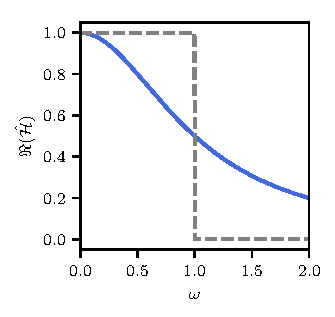
\includegraphics[scale=1]{S3_SFD_transfer_function}
      \caption{Evolution of $\Re \left( \hat{\mathcal{H}} \right)$ ({\color{blue} ---}), i.e.\ the real part of the Laplace transform of the exponential filter, as a function of the frequency $\omega$ for $\Delta=1$. The gray dashed line depicts the ideal spectral cutoff filter.}
      \label{fig: numerics -- lapalce transform}
    \end{figure}

    %-----> Newton-Krylov method.
    \subsubsection{Newton-Krylov methods}
    \label{subsubsec: numerics -- newton-krylov methods}

    While we relied on the continuous time representation of our system in \textsection \ref{subsubsec: numerics -- selective frequency damping}, we will now turn to its discrete-time counterpart in order to stay as close as possible to the actual time-stepper implementation of the algorithm to be describe. For that purpose, we will thus consider the following nonlinear system
    \begin{equation}
      \mathbf{X}_{k+1} = \mathbfcal{G}\left( \mathbf{X}_k \right).
      \label{eq: numerics -- discrete time system}
    \end{equation}
    Our goal is thus to find a fixed point $\mathbf{X}$ of this problem. Newton-Raphson method is a natural choice, provided the dimension of $\mathbf{X}$ is not too large. For large-scale dynamical systems, one may turn to the class of Newton-Krylov methods instead. These encompasses a wide variety of different approaches, part of which have been reviewed in \cite{jcp:knoll:2004}. In the rest of this section, we will present a variant of the recursive projection method originally proposed by Shroff \& Keller \cite{siam:shroff:1993}.

    % It can be shown that iteration \eqref{eq: numerics -- discrete time system} converges if all the eigenvalues $\{ \mu_k \}_1^n$ of the Jacobian of $\mathbfcal{G}$ lie in the unit disk and the initial iterate $\mathbf{X}_0$ is sufficiently close to the actual fixed point $\mathbf{X}^*$. Note moreover that, for our purposes, the Jacobian of $\mathbfcal{G}$ is given by the exponential propagator
    % \begin{equation}
    %   \mathbfcal{M} = \exp \left( \mathbfcal{A} T \right).
    %   \label{eq: numerics -- jacobian matrix}
    % \end{equation}
    % Iteration \eqref{eq: numerics -- discrete time system} will however fail to converge if any eigenvalues of $\mathbfcal{M}$ lies outside the unit disk. Moreover, if all eigenvalues are within the unit disk, convergence may be slow if any of them lie close to the boundary of the disk.

    %-----> BoostConv.
    \subsubsection{BoostConv}

    %-----> Comparison.
    \subsubsection{Comparison of the different approaches}


  %%%%%%%%%%%%%%%%%%%%%%%%%%%%%%%%%%%%%%%%%%%%
  %%%%%                                  %%%%%
  %%%%%     MODAL STABILITY ANALYSIS     %%%%%
  %%%%%                                  %%%%%
  %%%%%%%%%%%%%%%%%%%%%%%%%%%%%%%%%%%%%%%%%%%%

  \subsection{Linear stability and eigenvalue computation}

  The aim of linear stability analysis is to determine whether a perturbation $\textbf{x}$, governed by
  \begin{equation}
    \dot{ \mathbf{x} } = \mathbfcal{A} \mathbf{x},
    \notag
  \end{equation}
  will grow or decay exponentially rapidly as $t \to \infty$. This asymptotic behavior is entirely governed by the eigenspectrum of the Jacobian matrix $\mathbfcal{A}$: if at least one of its eigenvalues has a positive (resp. negative) real part, the linear system considered is unstable (resp. stable), see \textsection \ref{subsec: theory -- linear stability} for more details.

  It must emphasized that, within a time-stepper framework, one does not seek directly for the eigenpairs of the Jacobian matrix $\mathbfcal{A}$ of the continuous-time problem. Instead, the problem considered is recast in the discrete-time framework as
  \begin{equation}
    \mathbf{x}_{k+1} = \mathbfcal{M} \mathbf{x}_k,
    \label{eq: numerics -- discrete-time linear system}
  \end{equation}
  where $\mathbfcal{M} = \exp \left( \mathbfcal{A} T \right)$ is the exponential propagator already introduced in \textsection \ref{subsec: theory -- linear stability}, \textsection \ref{subsubsec: theory -- optimal perturbation}, and \textsection \ref{subsubsec: numerics -- newton-krylov methods}, and where $T$ is the sampling period. The system is then linearly unstable if at least one eigenvalue $\mu$ of $\mathbfcal{M}$ lies outside the unit disk, i.e. $\vert \mu \vert > 1$.

  As discussed previously, although one cannot explicitly assemble the exponential propagator $\mathbfcal{M}$, its action onto a given vector $\mathbf{x}_k$ simply amounts to march in time the linearized system from $t = kT$ to $t = (k+1)T$. This ability to evaluate relatively easily the matrix-vector product given by \eqref{eq: numerics -- discrete-time linear system} allows us to use iterative solvers as to compute the eigenpairs of $\mathbfcal{M}$. The rest of this section is thus devoted to the presentation of two iterative eigenvalue solvers, namely the Arnoldi decomposition and the Krylov-Schur decomposition.
    % %-----> Power Iteration.
    % \subsubsection{Power Iteration method}
    % \label{subsubsec: numerics -- power iteration}

    %-----> Arnoldi decomposition.
    \subsubsection{Arnoldi decomposition}
    \label{subsubsec: numerics -- arnoldi}

    Let us denote the following sequence of vectors
    \begin{equation}
      \mathbfcal{K}_m\left( \mathbfcal{M}, \mathbf{v}_0 \right) = \left\{ \mathbf{v}_0, \mathbfcal{M}\mathbf{v}_0, \cdots, \mathbfcal{M}^{m-1} \mathbf{v}_0 \right\}.
      \label{eq: numerics -- krylov sequence}
    \end{equation}
    Eq. \eqref{eq: numerics -- krylov sequence} is known as a \emph{Krylov sequence} eventually converging toward the eigenvector associated to the largest eigenvalue (in modulus) of $\mathbfcal{M}$ as $m \to \infty$. Generating this sequence to approximate the leading eigenpair of $\mathbfcal{M}$ is known as the \emph{power iteration method}. Note that this simple method retains only the last vector of this sequence while discarding the information contained in the first $m-1$ vectors.

    Contrary to the power iteration method, Arnoldi decomposition uses all of the information contained in the Krylov sequence \eqref{eq: numerics -- krylov sequence} as to compute better estimates of the leading eigenvalues of $\mathbfcal{M}$. Readers can easily be convinced that the Krylov sequence \eqref{eq: numerics -- krylov sequence} obeys
    \begin{equation}
      \mathbfcal{M} \mathbfcal{K}_m \simeq \mathbfcal{K}_m \mathbfcal{C},
      \notag
    \end{equation}
    where $\mathbfcal{C}$ is a $m \times m$ companion matrix representing the low-dimensional projection of $\mathbfcal{M}$ onto the span of the Krylov sequence \eqref{eq: numerics -- krylov sequence}. As such, the eigenpairs of $\mathbfcal{C}$ approximate the leading eigenpairs of $\mathbfcal{M}$. It must be emphasized however that, as $m$ increases, the last vectors in the Krylov sequence become almost parallel. Consequently, the companion matrix $\mathbfcal{C}$ becomes increasingly ill-conditioned. As to overcome the loss of information from the power iteration method and the increasingly ill-conditioned companion matrix decomposition, the Arnoldi method combines them with a Gram-Schmidt orthogonalization process. The basic Arnoldi iteration then reads
    \begin{equation}
      \mathbfcal{MV}_m = \mathbfcal{V}_m \mathbfcal{H}_m + \mathbf{r}_{m} \mathbf{e}^T_m,
      \label{eq: numerics -- m-step Arnoldi}
    \end{equation}
    where $\mathbfcal{V}_m$ is an orthonormal set of vectors, $\mathbfcal{H}_m$ is a $m \times m$ upper Hessenberg matrix and $\vert \mathbf{r}_{m} \mathbf{e}^T_m \vert$ is the residual indicating how far $\mathbfcal{V}_m$ is from from an invariant subspace of $\mathbfcal{M}$. Because of its relatively small dimension, the eigenpairs $\left( \mu_H, \mathbf{y} \right)$ of the Hessenberg matrix, also known as Ritz pairs, can be computed using direct eigensolvers, e.g.\ QZ decomposition. The Ritz pairs of $\mathbfcal{H}_m$ are related to the eigenpairs of $\mathbfcal{M}$ as follows
    \begin{equation}
      \begin{aligned}
        \mu_{\mathbfcal{M}} & \simeq \mu_{\mathbfcal{H}} \\
        \hat{\mathbf{u}} & \simeq \mathbfcal{V}_m \mathbf{y}.
      \end{aligned}
    \end{equation}
    A detailed presentation of the basic $m$-step Arnoldi factorization is given in algorithm \eqref{algo: Arnoldi} while figure \ref{fig: numerics -- arnoldi decomposition} depicts its block-diagram representation to ease the understanding. As can be seen, Arnoldi decomposition is relatively simple to implement within an existing time-stepper code. One has to bear in mind however that this technique resembles some sophisticated signal processing. As a consequence, in order to capture (within a time-stepper framework) an eigenpair of the Jacobian matrix $\mathbfcal{A}$ characterized by a circular frequency $\omega$, one has to obey the Nyquist criterion and needs at least four snapshots to appropriately discretize the associated period.

    \begin{algorithm}
      \begin{algorithmic}
        \REQUIRE $\mathbfcal{M} \in \mathbb{R}^{n \times n}$, starting vector $\mathbf{v} \in \mathbb{R}^n$.\\
        $\mathbf{v}_1 = \mathbf{v} / \| \mathbf{v} \|$;\\
        $\mathbf{w} = \mathbfcal{M} \mathbf{v}_1$; \\
        $\alpha_1 = \mathbf{v}_1^T \mathbf{w}$;\\
        $\mathbf{f}_1 \leftarrow \mathbf{w} - \alpha_1 \mathbf{v}_1$;\\
        $\mathbfcal{V}_1 \leftarrow \left( \mathbf{v}_1 \right)$; \\
        $\mathbfcal{H}_1 \leftarrow (\alpha_1)$;\\
        \FOR{$j=1,2,\cdots,m-1$}
        \STATE{$\beta_j=\|\mathbf{f}_j\|$; \\
        $\mathbf{v}_{j+1} \leftarrow \mathbf{f}_j/\beta_j$; \\
        $\mathbfcal{V}_{j+1} \leftarrow \left( \mathbfcal{V}_j, \mathbf{v}_{j+1} \right)$;\\

        $\hat{\mathbfcal{H}}_j \leftarrow \begin{pmatrix}
                                            \mathbfcal{H}_j \\
                                            \beta_j \mathbf{e}_j^T
                                          \end{pmatrix}
        $ \\
        $\mathbf{w} \leftarrow \mathbfcal{M} \mathbf{v}_{j+1}$;\\
        $\mathbf{h} \leftarrow \mathbfcal{V}_{j+1}^T \mathbf{w}$; \\
        $\mathbf{f}_{j+1} \leftarrow \mathbf{w} - \mathbfcal{V}_{j+1} \mathbf{h}$;\\
        $\mathbfcal{H}_{j+1} \leftarrow (\hat{\mathbfcal{H}}_j,\mathbf{h})$;}
        \ENDFOR
      \end{algorithmic}
      \caption{The $m$-step \emph{Arnoldi} factorisation.}
      \label{algo: Arnoldi}
    \end{algorithm}

    \begin{figure}[b]
      \centering
      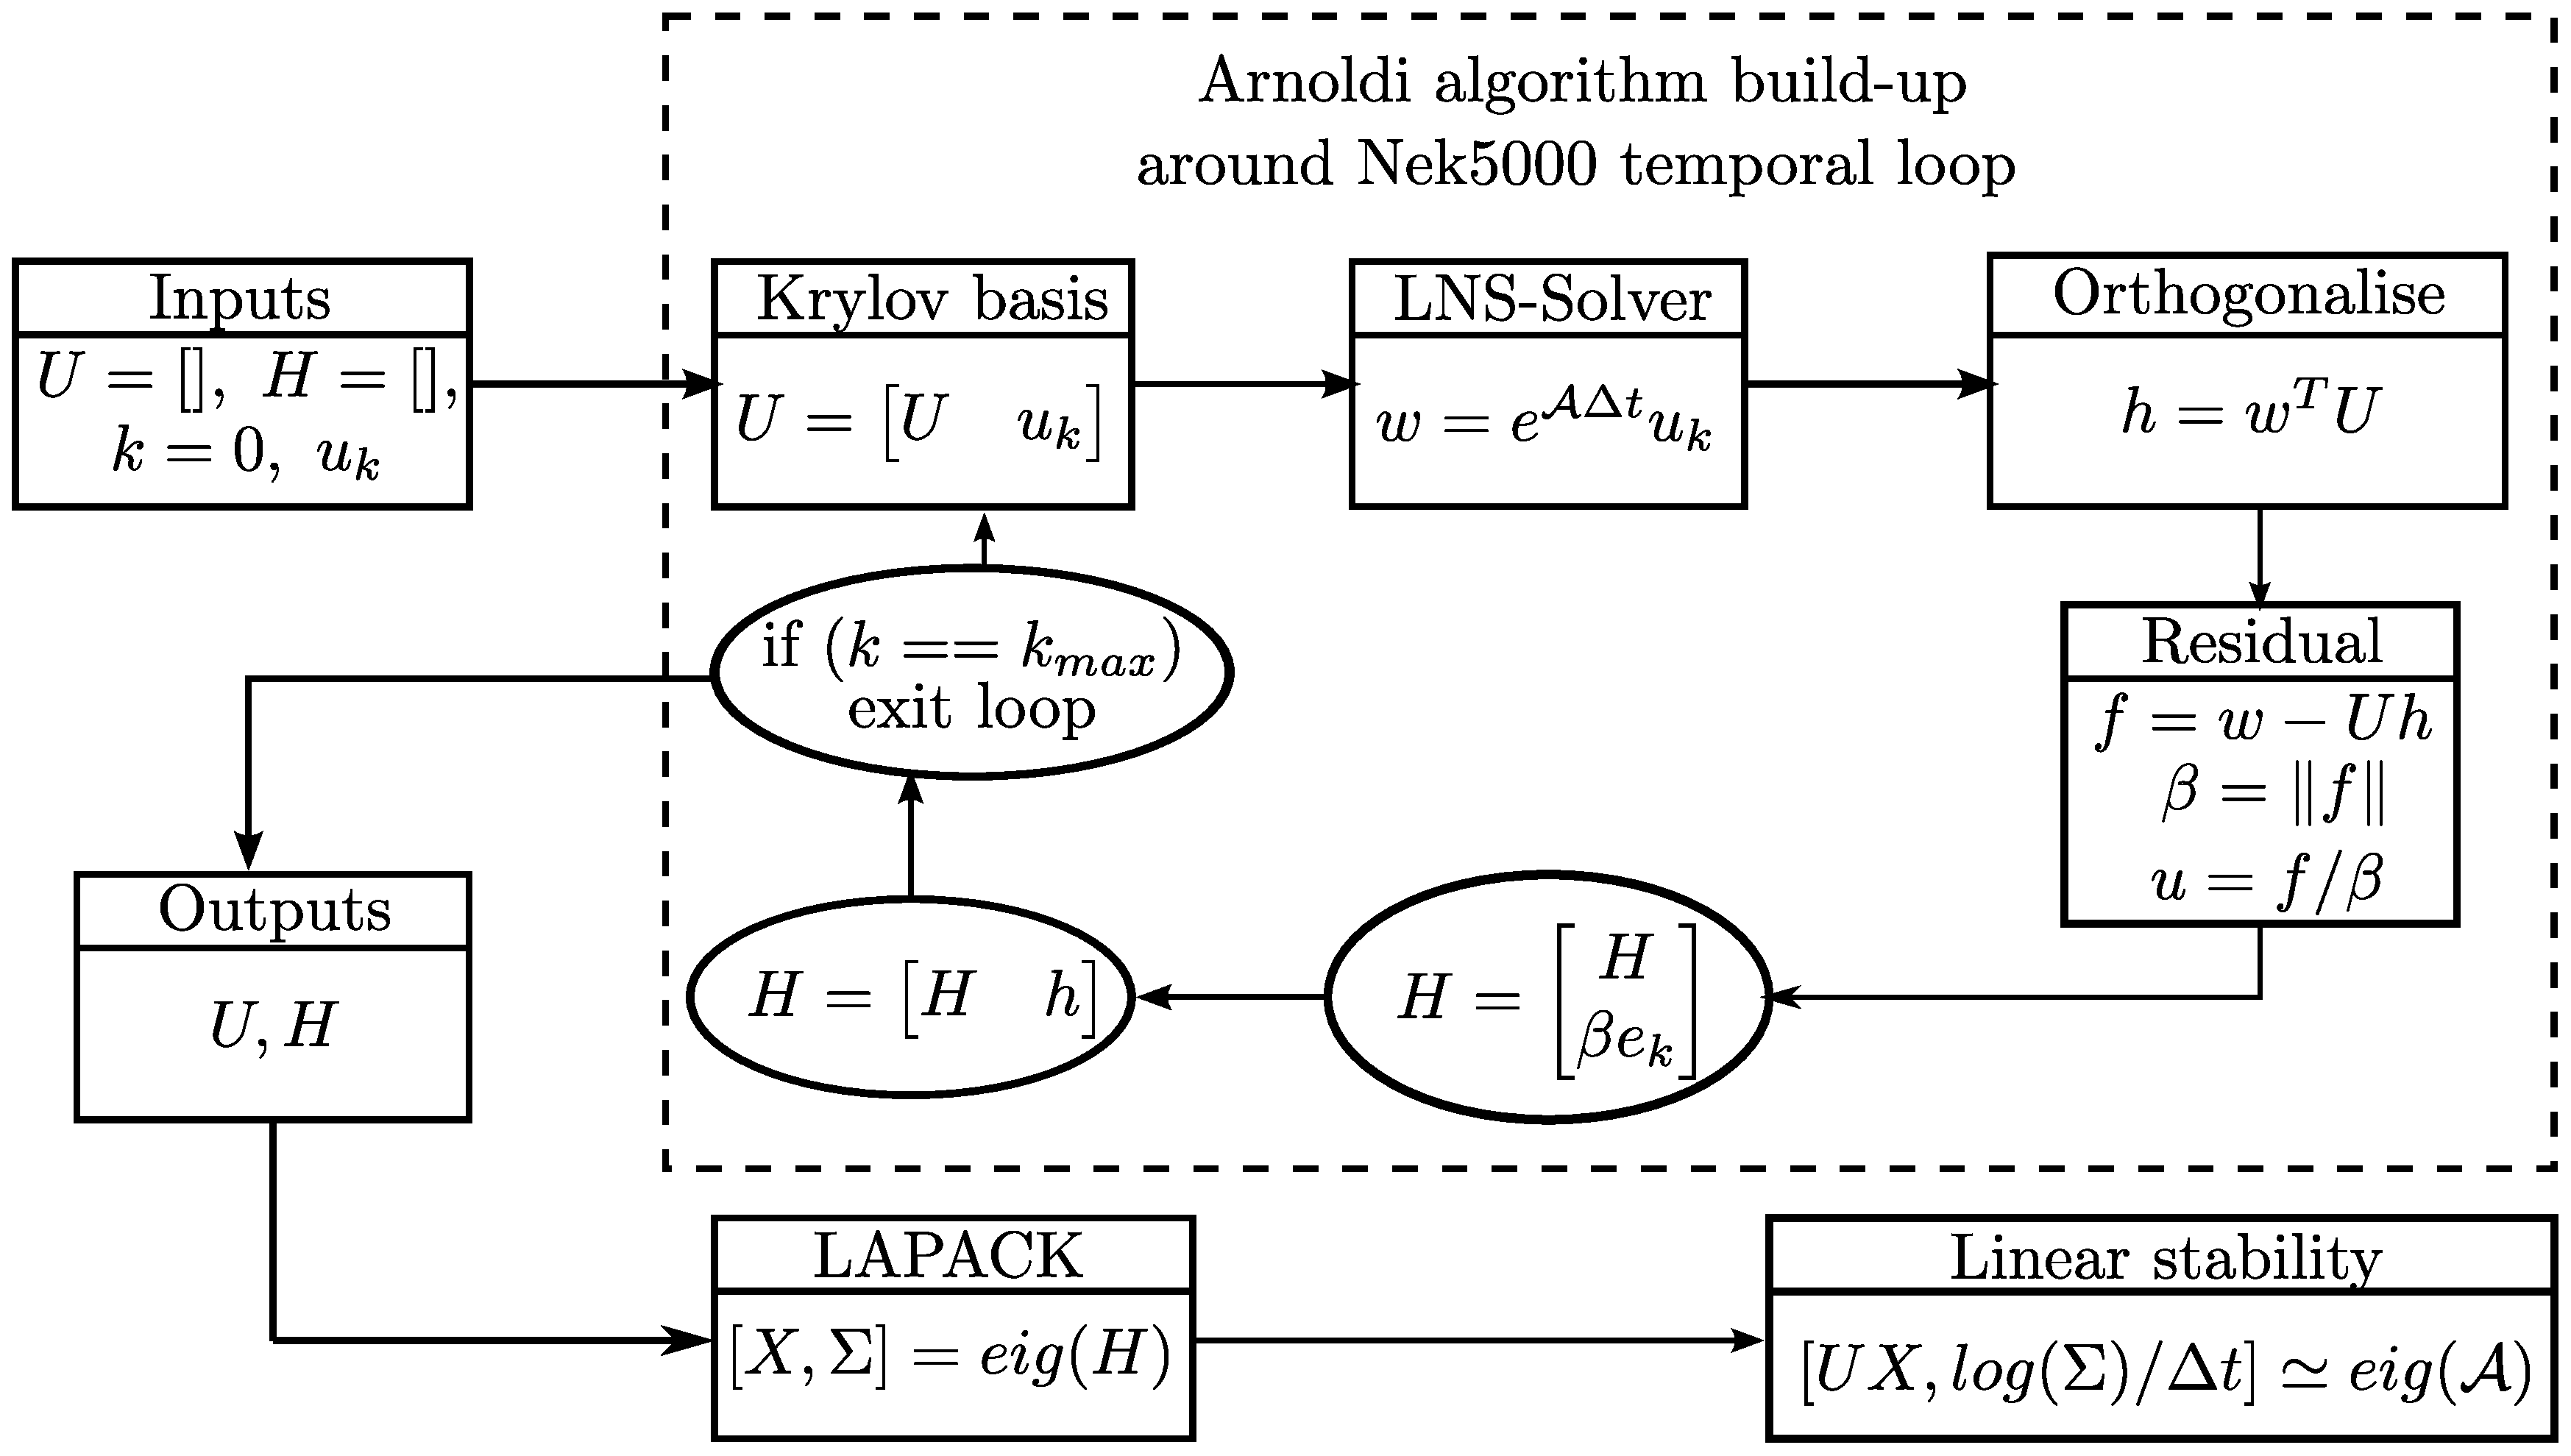
\includegraphics[width=.9\textwidth]{Arnoldi}
      \caption{Block-diagram representation of the basic $m$-step Arnoldi factorization. Note that, within a time-stepper framework, every matrix-vector product $\mathbfcal{M} \mathbf{v}_i$ is evaluated by marching in time the linearized system considered.}
      \label{fig: numerics -- arnoldi decomposition}
    \end{figure}

    %-----> Krylov-Schur decomposition.
    \subsubsection{Krylov-Schur decomposition}

    Let us consider the $m$-step Arnoldi factorization
    \begin{equation}
      \mathbfcal{MV}_m = \mathbfcal{V}_m \mathbfcal{H}_m + \beta \mathbf{v}_{m+1} \mathbf{e}^T_m
      \label{eq: m-step Arnoldi}
    \end{equation}
    introduced in \textsection \ref{subsubsec: numerics -- arnoldi}. As discussed previously, the Ritz pair $\left( \mu_H, \mathbfcal{V}_m \mathbf{y} \right)$ of $\mathbfcal{H}_m$ provides a good approximation for the eigenpair $\left( \mu, \hat{\mathbf u} \right)$ of the matrix $\mathbfcal{M}$. One limitation of the Arnoldi decomposition is however that the dimension $m$ of the Krylov subspace necessary to converge the leading Ritz pairs is not known \emph{a priori}. It might hence be relatively large, thus potentially causing some numerical and/or practical problems (e.g.\ storage of Krylov basis $\mathbfcal{V}_m$, forward instability of the Gram-Schmidt process involved in the Arnoldi decomposition, etc). Two different approaches have been proposed to overcome these limitations: the \emph{Implicitly Restarted Arnoldi Method} introduced by Sorensen \cite{Sorensen_SIAM_1992} in 1992 and the \emph{Krylov-Schur decomposition} introduced by Stewart \cite{Stewart_SIAM_2001} in 2001. In the present work, the latter approach has been preferred because of its simplicity of implementation and its robustness.

    The Krylov-Schur method is based on the generalization of the m-step Arnoldi factorization~\eqref{eq: m-step Arnoldi} to a \emph{Krylov decomposition} of order $m$
    \begin{equation}
      \mathbfcal{MV}_m = \mathbfcal{V}_m \mathbfcal{B}_m + \mathbf{v}_{m+1} \mathbf{b}_{m+1}^T
      \label{eq: Krylov decomposition}
    \end{equation}
    in which the matrix $\mathbfcal{B}_m$ and the vector $\mathbf{b}_{m+1}$ have no restriction. The Arnoldi decomposition then appears as a special case of Krylov decomposition when $\mathbfcal{B}_m$ is restricted to be in upper Hessenberg form and $\mathbf{b}_{m+1} = \mathbf{e}_m$. Another special case is the \emph{Krylov-Schur} decomposition in which the matrix $\mathbfcal{B}_m$ is in real Schur form (i.e.\ quasi-triangular form with its eigenvalues in the $1 \times 1$ or $2 \times 2$ diagonal blocks). It has been shown by Stewart \cite{Stewart_SIAM_2001} that Krylov and Arnoldi decompositions are equivalent (i.e.\ they have the same Ritz approximations). Moreover, by means of orthogonal similarity transformations, any Krylov decomposition can be transformed into an equivalent Krylov-Schur decomposition. The core of the Krylov-Schur method is thus based on a two-steps procedure: (\emph{i}) an expansion step performed using a $m$-step Arnoldi factorization, and (\emph{ii}) a contraction step to a Krylov-Schur decomposition of order $p$ retaining only the most useful spectral information from the initial $m$-step Arnoldi decomposition. Given an initial unit-norm vector $\mathbf{v}_1$, a subroutine to compute the matrix-vector product $\mathbfcal{M} \mathbf{v}_i$, and the desired dimension $m$ of the Krylov subspace, the Krylov-Schur method can be summarized as follows:
    \begin{enumerate}
      \item Construct an initial Krylov decomposition of order $m$ using for instance the $m$-step Arnoldi factorization~\eqref{eq: m-step Arnoldi}.

      \item Check for the convergence of the Ritz eigenpairs. If a sufficient number has converged, then stop. Otherwise, proceed to step 3.

      \item Compute the real Schur decomposition $\mathbfcal{B}_m = \mathbfcal{Q} \mathbfcal{S}_m \mathbfcal{Q}^T$ such that the matrix $\mathbfcal{S}_m$ is in real Schur form and $\mathbfcal{Q}$ is the associated matrix of Schur vectors. It is assumed furthermore that the Ritz values on the diagonal blocks of $\mathbfcal{S}_m$ have been sorted such that the $p$ ''wanted'' Ritz values are in the upper-left corner of $\mathbfcal{S}_m$, while the $m-p$ ''unwanted'' ones are in the lower-right corner. At this point, we have the following re-ordered Krylov-Schur decomposition
      \begin{equation}
        \mathbfcal{M} \tilde{\mathbfcal{V}}_m =
        \tilde{\mathbfcal{V}}_m
        \begin{bmatrix}
         \mathbfcal{S}_{11} & \mathbfcal{S}_{12} \\
         {\mathbf 0}     & \mathbfcal{S}_{22}
       \end{bmatrix}
       + {\mathbf v}_{m+1}\begin{bmatrix}
                           {\mathbf b}_{1}^T & {\mathbf b}_{2}^T
                           \end{bmatrix}
        \label{eq: Krylov-Schur decomposition}
      \end{equation}
      with $\tilde{\mathbfcal{V}}_m = \mathbfcal{V}_m  \mathbfcal{Q}$ being the re-ordered Krylov basis, $\mathbfcal{S}_{11}$ the subset of the Schur matrix containing the $p$ ''wanted'' Ritz values, $\mathbfcal{S}_{22}$ the subset containing the $m-p$ ''unwanted'' ones, and $\begin{bmatrix} {\mathbf b}_1^T & {\mathbf b}_2^T \end{bmatrix} = {\mathbf b}^T \mathbfcal{Q}$.

      \item Truncate the Krylov-Schur decomposition~\eqref{eq: Krylov-Schur decomposition} of order $m$ to a Krylov decomposition of order $p$,
        \begin{equation}
          \mathbfcal{M}\tilde{\mathbfcal{V}}_p = \tilde{\mathbfcal{V}}_p \mathbfcal{S}_{11} + \tilde{\mathbf v}_{p+1}{\mathbf b}_1^T
        \end{equation}
      with $\tilde{\mathbfcal{V}}_p$ equal to the first $p$ columns of $\tilde{\mathbfcal{V}}_m$ and $\tilde{\mathbf v}_{p+1} = {\mathbf v}_{m+1}$.

      \item Extend again to a Krylov decomposition of order $m$ using a variation of the procedure used in the first step: the procedure is re-initialized with the starting vector ${\mathbf v}_{p+1}$ but all the vectors in $\tilde{\mathbfcal{V}}_p$ are taken into account in the orthogonalization step.

      \item Check the convergence of the Ritz values. If not enough Ritz values have converged, restart from step 3.

    \end{enumerate}
    This algorithm has two critical steps. The first one is the choice of the ''wanted'' Ritz values in the re-ordering of the Schur decomposition in step 2. Since we are only interested in the leading eigenvalues of the linearized Navier-Stokes operator, all the Ritz pairs being classified as ''wanted'' must satisfy $\left| \mu_w \right| \ge 1 - \delta$ (with $\delta = 0.05 - 0.1$ usually). Regarding the criterion assessing the convergence of a given Ritz pair, starting from the Krylov decomposition~\eqref{eq: m-step Arnoldi}, one can write
    \begin{equation}
      \| \mathbfcal{M} \mathbfcal{V}_m \mathbf{y} - \mathbfcal{V}_m \mathbfcal{B}_m \mathbf{y} \| = \| \mathbfcal{M} \mathbfcal{V}_m \mathbf{y} - \mu_{\mathbf B} \mathbfcal{V}_m \mathbf{y} \| = \left| \beta \mathbf{e}_m^T \mathbf{y} \right|
      \label{eq: Krylov convergence}
    \end{equation}
    with $(\mu_{\mathbf B},\mathbf{y})$ a given eigenpair of the matrix $\mathbfcal{B}_m$. If the right hand side $\left| \beta {\mathbf e}_{m}^T{\mathbf y} \right|$ is smaller than a given tolerance, then the Ritz pair $(\mu_{\mathbf B}, \mathbfcal{V}_m {\mathbf y})$ provides a good approximation to the eigenpair $(\mu, \hat{\mathbf u})$ of the original matrix $\mathbfcal{M}$. A Ritz value is generally considered as being converged if the associated residual $\left| \beta {\mathbf e}_{m}^T{\mathbf y} \right| \le 10^{-6}$.

    %-----> Comparisons.
    \subsubsection{Comparison of the two approaches}

  %%%%%%%%%%%%%%%%%%%%%%%%%%%%%%%%%%%%%%%%%%%%%%%%
  %%%%%                                      %%%%%
  %%%%%     NON-MODAL STABILITY ANALYSIS     %%%%%
  %%%%%                                      %%%%%
  %%%%%%%%%%%%%%%%%%%%%%%%%%%%%%%%%%%%%%%%%%%%%%%%

  \subsection{Non-modal stability and singular value decomposition}

    %-----> Optimal perturbation.
    \subsubsection{Optimal perturbation analysis}

    %-----> Resolvent analysis.
    \subsubsection{Resolvent analysis}
